\section{Out-of-Distribution Detection}
\label{sec:bkdg-ooddetect}

%(ood detection task definition)

%An ID training set $\mathcal{D}_{ID} = \{(\mathbf{x}_i, y_i)\}^{N}_{i=1}$ contains samples $x_i \in \mathcal{X}_{ID}$ and associated labels $y_i \in \mathcal{Y}_{ID} = \{1,2,\dots,C\}$ drawn from an ID distribution $P_{ID}(X, Y)$, i.e. $\mathcal{D}_{ID} \sim P_{ID}$. In the open-world problem setting, an OOD space also exists $\mathcal{D}_{OOD} = \{(\mathbf{x}_i), y_i\}^{L}_{i=1}$ with corresponding samples $x_i \in \mathcal{X}_{OOD}$ and some unknown OOD label $y_i \in \mathcal{Y}_{OOD} = \{y | y \notin \mathcal{Y}_{ID}\}$, drawn from OOD distribution $P_{OOD}(X, Y)$. Given a test sample $x'$, the goal of OOD detection is to identify if the test label $y' \in \mathcal{Y}_{ID}$ or $y' \in \mathcal{Y}_{OOD}$. A classification model $f$ is used as an OOD detector model $G$ in the following formulation
%\begin{equation}
%  G(x', f) =
%  \begin{cases}
%    1 \text{\ (OOD),} & \text{$S(x'; f) \geq \lambda$} \\
%    0 \text{\ (ID),} & \text{$S(x'; f) < \lambda$} \\
%  \end{cases}
%\end{equation}
%where $S$ is a scoring function and $\lambda$ is a threshold. In research, the threshold is often not used in evaluation as it depends on the application. Instead, a ranking is produced based on the $S$ scores to measure the Area Under the Receiver Operating Characteristic curve (AUROC). 

%For $\mathcal{D}_{id}$, the input space is denoted as $\mathcal{X}$ and the space of all ID class labels is given as $\mathcal{Y} = \{1, 2, ... , R\}$, where $R$ is the number of classes. The ID dataset $\mathcal{D}_{id}$ is drawn \emph{i.i.d.} from the joint data distribution $P_{\mathcal{X} \mathcal{Y}}$. Let the ID distribution $\mathcal{P}_{id}$ be the marginal distribution of $P_{\mathcal{X} \mathcal{Y}}$ on $\mathcal{X}$. Given \emph{only} $\mathcal{D}_{id}$, an OOD detection model detects if an input image data sample $x'$ is from the ID distribution $\mathcal{P}_{id}$ or not (i.e. the data sample is from the OOD distribution containing all other data samples). Typically, this detection is represented using a decision $G_{\lambda}(x)$, formulated as a level set estimation:
%\begin{equation}
%\begin{aligned}
%  G_{\lambda}(x) =
%  \begin{cases}
%        \text{ID}     & M(x) \geq \lambda \\
%        \text{OOD}    & M(x) < \lambda \\
%  \end{cases}
%\end{aligned}
%\end{equation}
%with OOD score $M(x)$ for sample $x$ and user-defined threshold $\lambda$. However, the OOD detection literature more frequently makes use of the area under the receiver operating characteristic (AUROC) score \cite{bradley1997use,hendrycks2017baseline,lee2018simple} to eliminate reliance on a threshold \cite{hendrycks2017baseline}. In this case, the AUROC score is constructed using the OOD score $M(x)$ for sample $x$ and label $1$ for ID data samples and $0$ for OOD data samples. In this paradigm (and henceforth in this proposal), the OOD score $M(x)$ is \textit{higher} for samples identified as \textit{more ID} and $M(x)$ is \textit{lower} for samples identified as \textit{more OOD}. %\textcolor{blue}{explicitly say that higher is less ood and vice versa?}
An ID training dataset $\mathcal{D}_{ID} = \{(x_i, y_i)\ |\ x_i \in \mathcal{x}_{ID},y_i \in \mathcal{Y}_{ID}\}_{i=1}^N$ is composed of samples $x_i \in \mathcal{X}_{ID}$ and labels $y_i \in \mathcal{Y}_{ID} = \{1,2,\dots,C\}$ for number of ID samples $N$ and number of ID classes $C$. $\mathcal{D}_{ID}$ is drawn \emph{i.i.d.} from an ID distribution $P_{ID}(X, Y)$, i.e. $\mathcal{D}_{ID} \sim P_{ID}$, which is the marginal distribution of joint data distribution $P_{\mathcal{X} \mathcal{Y}}$ on $\mathcal{X}_{ID}$. There also exists the OOD marginal distribution $P_{OOD}$ on OOD data $\mathcal{X}_{OOD}$ and unknown OOD labels $\mathcal{Y}_{OOD}$. An OOD dataset $\mathcal{D}_{OOD} = \{(x_i)\ |\ x_i \in \mathcal{X}_{OOD},y_i \in \mathcal{Y}_{OOD}\}^{L}_{i=1}$ is drawn from the OOD distribution $\mathcal{D}_{OOD} \sim P_{OOD}$ and contains samples $x_i \in \mathcal{X}_{OOD}$ with labels $y_i \in \mathcal{Y}_{OOD} = \{y | y \notin \mathcal{Y}_{ID}\}$ for number of OOD samples $L$.

The OOD detection task is, given \emph{only} $\mathcal{D}_{ID}$ and a test sample $x'$, identify if the test label $y' \in \mathcal{Y}_{ID}$ or $y' \in \mathcal{Y}_{OOD}$. An OOD detection model $G$ uses an ML model $f$ in the following formulated level set estimation:
\begin{equation}
  G(x', f) =
  \begin{cases}
    1 \text{\ (OOD),} & \text{$S(x'; f) \geq \lambda$} \\
    0 \text{\ (ID),} & \text{$S(x'; f) < \lambda$} \\
  \end{cases}
\end{equation}
for scoring function $S(\cdot)$ and user-defined threshold $\lambda$. Of note is that the OOD score $S$ is \textit{higher} for samples identified as \textit{more ID} and $S$ is \textit{lower} for samples identified as \textit{more OOD}.

%{\color{red}near- vs far-OOD definitions or explanation}

\section{Metrics}
%However, the OOD detection literature more frequently makes use of the area under the receiver operating characteristic (AUROC) score \cite{bradley1997use,hendrycks2017baseline,lee2018simple} to eliminate reliance on a threshold \cite{hendrycks2017baseline}. In this case, the AUROC score is constructed using the OOD score $M(x)$ for sample $x$ and label $1$ for ID data samples and $0$ for OOD data samples. In this paradigm (and henceforth in this proposal), the OOD score $M(x)$ is \textit{higher} for samples identified as \textit{more ID} and $M(x)$ is \textit{lower} for samples identified as \textit{more OOD}.
Several metrics have been proposed to measure the performance of OOD detection methods \cite{lu2024recent}:
\begin{itemize}
    \item \textbf{Area Under the Receiver Operating Characteristic Curve (AUC).} This metric quantifies the model likelihood of assigning higher scores to ID samples with respect to scores of OOD samples. AUC correlates with the model's ability to correctly rank ID samples higher than OOD samples. A \textbf{higher} AUC is indicative of better OOD detection performance.
    \item \textbf{False Positive Rate at 95\% True Positive Rate (FPR95).} This metric quantifies the false positive rate (FPR) at the value where the true positive rate (TPR) becomes 95\%. It measures the amount of OOD samples incorrectly classified as ID. FPR95 correlates with an OOD detection model's likelihood of false detections under strict ID detection requirements. A \textbf{lower} FPR95 is indicative of better OOD detection performance.
    \item \textbf{Area Under the Precision-Recall Curve (AUPR).} This metric quantifies a combination of model precision and recall. Two versions of AUPR exist: one where precision and recall is considered for ID data as the ``correct'' class of interest (AUPR-IN) and one where OOD data is considered as the ``correct'' class of interest (AUPR-OUT). AUPR is particularly effective at measuring OOD detection performance under severe ID-OOD data imbalance. AUPR correlates directly with the model's ability to correctly classify ID (or OOD) data. A \textbf{higher} AUPR is indicative of better OOD detection performance.
    %\item \textbf{Detection Error (DE).} This metric quantifies a combination of model precision and recall. Two versions of AUPR exist: one where precision and recall is considered for ID data as the ``correct'' class of interest (AUPR-IN) and one where OOD data is considered as the ``correct'' class of interest (AUPR-OUT). In particular, AUPR effectively measures OOD detection performance under severe ID-OOD data imbalance. AUPR correlates directly with the model's ability to correctly classify ID (or OOD) data. A \textbf{higher} AUPR is indicative of better OOD detection performance.
\end{itemize}

Of note is that the OOD detection literature more frequently makes use of the AUC score \cite{bradley1997use,hendrycks2017baseline,lee2018simple}. AUC covers general model performance and avoids reliance on a user-defined threshold which may be application- or domain-dependent \cite{hendrycks2017baseline}. This thesis likewise prioritizes AUC as the predominant OOD detection metric but other metrics are reported in varying capacities as needed to illustrate robustness.

\section{Relevant OOD Detection Methods}

\subsection{Maximum Softmax Probability}

The paper proposing Maximum Softmax Probability (MSP) \cite{hendrycks2017baseline} is widely considered to be the work spawning the OOD Detection field. MSP uses a classification model $f$ and treats the predicted probability distribution, $\text{softmax}(\hat{y})$, as a representation of model confidence in the sample $x$ under consideration, where ``$\text{softmax}$'' is the softmax function and $\hat{y} = f(x) \in \mathbb{R}^C$ is the predicted logits. The maximum probability is used as the OOD score
\begin{equation}
\begin{aligned}
    S_{MSP}(x,f) = \max_c\ \text{softmax}(f(x)), \\
\end{aligned}
\end{equation}
with $\max\limits_{c}$ indicating the maximum function over probabilities of classes $c \in C$. MSP stands as a simple OOD detection tool that remains as a reliable baseline, although much research has revealed limitations to the method \cite{hendrycks2019scaling} and proposed improvements \cite{sun2021react}.

\subsection{Mahalanobis Distance}
\label{sec:bkgd-md}

%The MD OoD score measures the distance between a sample and a Gaussian distribution. Maximum likelihood estimation is used to approximately fit class-conditional Gaussian distributions to each class in the training distribution. The empirical class means $\hat{\mu}_{c}$ and covariance matrix $\hat{\Sigma}$ are calculated from the training dataset $\mathcal{D}_{id}$ using some feature extractor $\phi$
%\begin{equation}
%\begin{aligned}
%    \hat{\mu}_{c} & = \frac{1}{N_{c}} \sum_{i:y_{i}=c} \phi(x_{i}) \\
%    \hat{\Sigma} & = \frac{1}{N} \sum_{c} \sum_{i:y_{i}=c} (\phi(x_{i}) - \hat{\mu}_{c}) (\phi(x_{i}) - \hat{\mu}_{c})^\top \\
%\end{aligned}
%\end{equation}
%where $N_{c}$ is the number of samples in class $c$. For \sysa, the feature extractor $\phi$ is replaced with the MVCNN pipeline, using the fused feature $z_{fused}$ to construct the empirical class means and covariance matrix. Given a test instance $x'$, \sysa extracts the test fused feature $z'_{fused} = \mathcal{G} (\Phi_{V}(x'_{V}), s) $ ($V = \{org, fg, bg\}$) and computes the distance between it and the nearest class-conditional Gaussian distribution, resulting in the final MD OoD score
%\begin{equation}
%\begin{aligned}
%     M_{MD}(x') = \max_{c} (-(z_{fused}' - \hat{\mu}_{c})^\top \hat{\Sigma}^{-1} (z_{fused}' - \hat{\mu}_{c})) \\
%\end{aligned}
%\end{equation}
Mahalanobis Distance (MD) \cite{lee2018simple} is considered the original distance-based OOD detection method, measuring the distance between a sample $x$ and Gaussian distributions representing ID data in the feature space. MD first computes class-conditional Gaussian distributions for each ID class in the training distribution. This is intractable as it cannot be assumed that any model has access to the entire ID training data distribution. The authors of MD propose instead to approximately fit the ID class Gaussian distributions using maximum likelihood estimation over the available training data and tied covariance.

Specifically, empirical class means $\hat{\mu}_{C} = \{\hat{\mu}_{c}\}_{c=1}^{C}$ and a single, shared covariance matrix $\hat{\Sigma}$ are computed from the training dataset $\mathcal{D}_{id}$ using some feature extractor $\phi$
\begin{equation}
\begin{aligned}
    \hat{\mu}_{c} & = \frac{1}{N_{c}} \sum_{i:y_{i}=c} \phi(x_{i}) \\
    \hat{\Sigma} & = \frac{1}{N} \sum_{c} \sum_{i:y_{i}=c} (\phi(x_{i}) - \hat{\mu}_{c}) (\phi(x_{i}) - \hat{\mu}_{c})^\top. \\
\end{aligned}
\end{equation}
$N_{c}$ is the number of samples in class $c$ and sample $x_{i} \in \mathcal{D}_{ID}$.

Given the class means $\hat{\mu}_{C}$ and covariance matrix $\hat{\Sigma}$, the MD OOD score is calculated using the feature vector $z' = \phi(x')$ for test sample $x'$
\begin{equation}
\begin{aligned}
     S_{MD}(x',\phi) = \max_{c} (-(z' - \hat{\mu}_{c})^\top \hat{\Sigma}^{-1} (z' - \hat{\mu}_{c})). \\
\end{aligned}
\end{equation}
$\max\limits_{c}$ again indicates the maximum function over classes $c \in C$. MD continues to demonstrate impressive performance in many OOD detection domains \cite{yang2022openood,zhang2023openood,ren2021simple}. Importantly, as MD is a distance-based OOD detection method that relies on features (also referred to as a ``feature-based OOD detection method'' in this thesis), its performance on OOD detection improves as the embedded feature space (henceforth referred to simply as ``feature space'') improves. That is, as the model learns increasingly discriminative, ID class-relevant features, ID sample features cluster into localized groups (according to class) with increasingly distinct separation in the feature space. MD accurately models this feature space and thus separates OOD sample features from ID sample features more clearly \cite{lee2018simple,sun2022out,ammar2024neco,fort2021exploring}. Orthogonal techniques that improve learning of features from data, e.g. data augmentation, also benefit MD (and other feature-based OOD detection methods) \cite{sun2022out,khosla2020supervised,hendrycks2022pixmix,yun2019cutmix}.

\begin{figure}
 \centering
 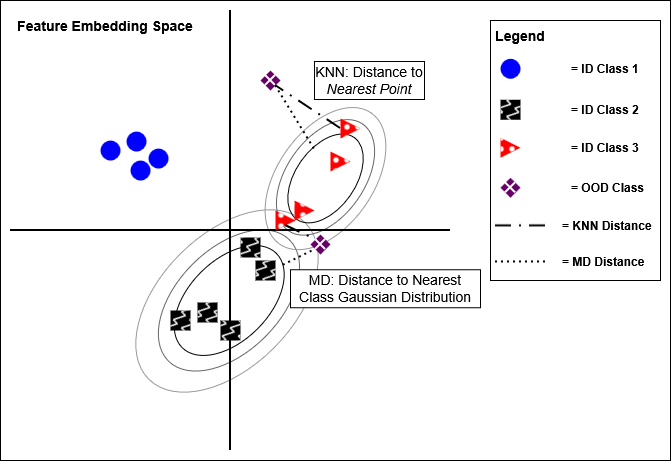
\includegraphics[width=0.9\linewidth]{figures/mdknn_example}
  \caption{Example illustration displaying the functionality of two distance-based OOD detection methods, namely MD and KNN, in the embedded feature space.
  }
  \label{fig:bkgd-mdknn}
\end{figure}

\subsection{k-Nearest Neighbors}

%The KNN OoD score is a non-parametric distance metric that uses the $k$-th nearest neighbor distance between a test image feature vector and feature vectors from the training dataset. Previous investigations have shown that the $L_{2}$ feature norms in ID data are larger than those from OoD data \cite{tack2020csi,huang2021importance}. To account for this, the feature vectors used by \sysa in the KNN score are the normalized fused features $\zeta = \frac{z_{fused}}{\lvert \rvert z_{fused} \lvert \rvert_{2}}$. Given normalized fused feature vectors $\mathbb{Z} = \{\zeta_{i}\}^{N}$ for the training dataset $\mathcal{D}_{id}$ and a test instance $x'$, the KNN OoD score is calculated as follows. First, the normalized fused feature vector $\zeta'$ for $x'$ is generated and the Euclidean distance of $x'$ from each $x_{i} \in \mathcal{D}_{id}$ is calculated as $\lvert \rvert \zeta_{i} - \zeta' \lvert \rvert_{2}$. Second, the features in $\mathbb{Z}$ are reordered according to distance to $\zeta'$, $\mathbb{Z}' = \{\zeta_{(i)}\}^{N}$. Finally, the KNN OoD score $M_{KNN}(x')$ for $x'$ is computed as the negation of the Euclidean distance to the $k$-th ID feature
%\begin{equation}
%\begin{aligned}
%    M_{KNN}(x') = -\lvert \rvert \zeta_{(k)} - \zeta' \lvert \rvert_{2}
%\end{aligned}
%\end{equation}
%Following the conventions of OoD scores (see Section \ref{sec:intro-relwork-ood}), higher (lower) scores $M_{MD}(x')$ and $M_{KNN}(x')$ for test instance $x'$ indicate the instance is less (more) OoD.
k-Nearest Neighbors (KNN) \cite{sun2022out} is another distance-based OOD detection method. However, it differs from MD in that it uses a non-parameteric distance metric. Specifically, KNN uses the $k$-th nearest neighbor distance between a sample $x$ and the training dataset feature vectors. An illustration of the similarities and differences between MD and KNN is in \ref{fig:bkgd-mdknn}.

ID training feature vectors are collected and normalized (per findings from a related investigation \cite{tack2020csi,huang2021importance}) from the training dataset $\mathcal{D}_{ID}$, $\mathcal{Z} = \{\zeta_{i}\}^{N}$ with $\zeta = \frac{z}{\lvert \rvert z \lvert \rvert_{2}}$ as the $L_2$ norm of feature vector $z$. The KNN OOD score is calculated using the normalized feature vector $\zeta'$ for test sample $x'$. Specifically, the Euclidean distances between $\zeta'$ and each $\zeta_i \in \mathcal{Z}$, $d_{KNN,i}(\zeta', \zeta_i) = \lvert \rvert \zeta_{i} - \zeta' \lvert \rvert_{2}$, is computed and ranked according to distance, $D_{KNN}' = \{d_{KNN,(i)}\}^{N}$ where $(i)$ represents the newly ordered position. The $k$-th Euclidean distance is used as the OOD score
\begin{equation}
\begin{aligned}
    S_{KNN}(x',\mathcal{Z},k) = -d_{KNN,(k)}(\zeta', \zeta_{(k)}). \\
\end{aligned}
\end{equation}
Note that KNN does not require the labels of the ID data, i.e. it is unsupervised. This has certain advantages in settings without guaranteed access to labeled data. As with MD, KNN improves as the feature space improves. Furthermore, KNN makes no assumptions about the distributions of data in the feature space.


\subsection{Virtual Logit Matching}

%ViM \cite{wang2022vim}, which has been shown highly effective \cite{zhang2023openood}. It divides a sample feature into a column subspace (CS) component and a null subspace (NS) component \cite{cook2020outlier,wang2022vim}. 
%ViM works as follows: Given the feature extractor $\phi$ of $f$, we define the feature $z = \phi(x)$ for input sample $x$. Further, the model $f$ can be retrieved as $f(x) = \mathbf{W} \phi(x) + \mathbf{b}$ with $\mathbf{W} \in \mathbb{R}^{d \times C}$ and $\mathbf{b} \in \mathbb{R}^{C}$ as the weight matrix and bias of a fully-connected layer. $d$ is the dimension of feature $z$. Following from ViM, the final fully-connected classification layer weight matrix $\mathbf{W}$ can be decomposed into a CS $W$ and an NS $W^{\perp}$. $W^{\perp}$ is unique in that it does not affect classification but it influences OOD detection due to the definition of NS. That is, the NS $W^{\perp} = \text{Nul} \mathbf{W}$ is the set of solutions satisfying $\mathbf{W} z = 0$. $z$ can be similarly decomposed into $z = z^{W^{\perp}} + z^{W}$ with $z^{W^{\perp}}$ and $z^{W}$ are projections of $z$ to the NS $W^{\perp}$ and CS $W$ respectively.
%Both ViM and NuSA observed that NS projections $z^{W^{\perp}}$ deviated significantly in OOD samples with respect to ID samples. NuSA exploited this observation by defining a score $\text{NuSA}(x) = \frac{\sqrt{\|z\| - \|z^{W^{\perp}}\|}}{\|z\|}$ and ViM defined a score $\text{ViM}(x) = \| z^{W^{\perp}} \|$ in comparison to predicted logits. However, both NuSA and ViM assume access to the sample feature $z$ and/or logits $\hat{y}$ to generate their respective OOD scores. 
%ViM observed that NS projections $z^{W^{\perp}}$ deviated significantly in OOD samples with respect to ID samples. ViM exploited this observation by defining a score $\text{ViM}(x) = \| z^{W^{\perp}} \|$ in comparison to predicted logits. However, ViM assumes access to the sample feature $z$ and logits $\hat{y}$ to generate the OOD score. 
Virtual Logit Matching (VIM) \cite{wang2022vim} is a hybrid OOD detection approach that uses both features and predicted logits to quantify an OOD score. VIM divides the feature vector $z$ of a sample $x$ into a column subspace (CS) component and a null subspace (NS) component before comparing the NS component to predicted logits $\hat{y}$.

The detailed procedure is as follows: given feature extractor $\phi$ of model $f$ and feature vector $z = \phi(x)$ for input sample $x$, the model can be further specified as $f(x) = W \phi(x) + b$ for classification linear layer weight matrix $W \in \mathbb{R}^{d \times C}$ and bias $b \in \mathbb{R}^{C}$, where $d$ is the dimension of feature vector $z \in \mathbb{R}^d$. $W$ can be decomposed into a CS $W_{cs}$ and an NS $W^{\perp}$. $W^{\perp}$ is unique in that it does not affect classification but it influences OOD detection due to the definition of NS. Specifically, the NS $W^{\perp} = \text{Nul}\ W$ is the set of solutions satisfying $W z = 0$. $z$ can be similarly decomposed into $z= z^{W^{\perp}} + z^{W_{cs}}$ with $z^{W^{\perp}}$ and $z^{W_{cs}}$ as projections of $z$ to the NS $W^{\perp}$ and CS $W_{cs}$ respectively.

NS projections $z^{W^{\perp}}$ in OOD samples deviate significantly with those in ID samples. To exploit this, VIM directly compares the NS projection with predicted logits. First, the NS projection is redefined as a virtual logit $\hat{y}_0 = \alpha \| z^{W^{\perp}} \|$, with $\alpha$ as a scaling parameter computed from virtual logits and maximum predicted logits of the ID data
\begin{equation}
\begin{aligned}
    \alpha = \frac{\sum_{i=1}^{N} \max_{j=1,\dots,C} \hat{y}_j^i}{\sum_{i=1}^{N} \| z^{W^{\perp}} \|}. \\
\end{aligned}
\end{equation}
Then, the virtual logit is concatenated to the predicted logits and a softmax is performed to retrieve the NS projection sample probability. The probability of the virtual logit is used as the OOD score
\begin{equation}
\begin{aligned}
    S_{VIM}(z,\hat{y}) = \frac{e^{\hat{y}_0}}{\sum_{i=1}^{N} e^{\hat{y}_i} + e^{\hat{y}_0}}. \\
\end{aligned}
\end{equation}
VIM has consistently shown state-of-the-art performance despite many later works proposing alternative approaches for OOD detection. The combination of feature and logits information increases the saliency of information for OOD detection in any given evaluated sample.

\section{Multi-View Processing}
\label{sec:bkgd-mvp}

%We segment each image $x$ in $\mathcal{D}_{id}$ into a foreground ($x_{fg}$) and a background ($x_{bg}$) view.  We still use the original image $x$ (from here notated as $x_{org}$ for clarity) as it contains integrated information. 
%The three views $x_{org}$, $x_{fg}$, $x_{bg}$ are fed to a view feature extractor 
%to learn features $z_{org}$, $z_{fg}$, $z_{bg}$. 
%
%Given the three views $x_{org}$, $x_{fg}$, $x_{bg}$ of image $x$, Each view $x_v$ (where $v \in \{org, fg, bg\}$) is fed to the ViT and its corresponding \textit{view-specific} Adapter at each block. The ViT and view-specific Adapter parameters for a view $v$ we denote as $\phi_{v}$ (with $\vec{\phi} = \{\phi_{org}, \phi_{fg}, \phi_{bg}\}$). The penultimate feature $z_v \in \mathbb{R}^{T \times d}$ is thus obtained via $z_v = \phi_v (x_v)$. 
%Finally, the three view features $z_{org}$, $z_{fg}$, and $z_{bg}$ are fused 
A multi-view dataset $\mathcal{D}_{MV} = \{(x_{MV,i}, y_i)\}$ contains set of labels $y_i$ and a set of associated multi-view samples $x_{MV,i}$. Each multi-view sample is composed of a set of \emph{views} $x_{MV,i} = \{x_{i,0}, x_{i,1}, \dots, x_{i,V}\}$ where $V$ is the number of views. Views are images, with each view being a copy of the original image under covariate or semantic shift (including no shift, i.e. the original image itself). That is, given some augmentation function introducing covariate or semantic shift $\mathcal{B}(\cdot)$, a view is defines as $x_{i,v} = \mathcal{B}(x_i)$ for original image $x_i$.% and with $v \in \mathbb{N}^V$.

Multi-view models process multi-view datasets by taking each view in a multi-view sample as input and calculating some representation coalescing information across the views as output. The multi-view model $f_{MV}$ may be considered as a set of individual-view models $f_{MV} = \{f_0, f_1, \dots, f_V\}$. Each view in a multi-view sample $x_{i,v}$ is processed by its corresponding individual-view model $f_v$. Note that  individual-view models can be the same, and thus shared. Outputs from each individual-view model are then coalesced in an operation referred to as ``\textbf{fusion}'', resulting in a collective output from the multi-view model $f_{MV}(x_{MV,i}) = \mathcal{U}(\{f_0(x_{i,0}),f_1(x_{i,1}),\dots,f_V(x_{i,V})\})$ for fusion operation (or embodying architectural module) $\mathcal{U}$.

\section{Prompting for OOD Detection}

%Since we aim to use verbal prompts only,
%we propose to extract the latent knowledge in LLMs for OOD detection using prompts to approximate the NS and CS of an input sample $x$ using tokens (words) generated by the LLM, following the prompts. Given a prompt template $\mathcal{P}$ and an input $x$, an input prompt is constructed $\mathcal{P} (x)$. A function $\text{Parse}_{\perp}(\cdot)$ is used to extract the set of tokens representing the approximate NS $\mathcal{T}_{\perp} = \{t_{\perp,1},t_{\perp,2},\dots,t_{\perp,n}\}$ and $\text{Parse}_{\mathcal{C}}(\cdot)$ is used to extract the set of tokens representing the approximate CS $\mathcal{T}_{\mathcal{C}} = \{t_{\mathcal{C},1},t_{\mathcal{C},2},\dots,t_{\mathcal{C},m}\}$ from the generated output of an LLM model $f_{LLM}$
%\begin{equation}
%\begin{split}
%	%\{z_{org+fg}, z_{org+bg}\} & = CVCA(z_{fg \rightarrow org}, z_{bg \rightarrow org})
%	\mathcal{T}_{\perp} & = g_{\perp} (x) = \text{Parse}_{\perp} (f_{LLM}(\mathcal{P} (x))) \\
%	\mathcal{T}_{\mathcal{C}} & = g_{\mathcal{C}} (x) = \text{Parse}_{\mathcal{C}} (f_{LLM}(\mathcal{P} (x))) \\
%\end{split}
%\end{equation}
%We share the prompt template and examples in Appendix \ref{sec:app-prompts}. Our proposed method for exploiting this verbalized form of decomposition-based OOD detection, \sys-ViM, uses two  phases.
A text dataset $\mathcal{D} = \{(x_{\text{text},i}, y_i)\}$ is composed of labels $y_i \in \mathcal{Y}_{ID}$ and text samples $x_{\text{text},i} \in \mathcal{X}_{\text{text}}$. Given a prompt template $\mathcal{P}$ and a text input $x_{\text{text}}$, a prompt $P$ is constructed $P = \mathcal{P}(x_{\text{text}})$ as input to a language model (LM), e.g. an LLM, for generation of a response to be used for OOD detection. Specifically, given prompt template $\mathcal{P}$, a parsing function $\text{Parse}(\cdot)$ is used to extract an OOD score $S$ from the output of LM $f_{LM}$
\begin{equation}
	S(x_{\text{text}},f_{LM}) = \text{Parse}(f_{LM}(\mathcal{P}(x_{\text{text}}))).
\end{equation}
The parsing function $\text{Parse}(\cdot)$ typically operates over the tokens generated from the LM $\mathcal{T} = f_{LM}(\mathcal{P}(x_{\text{text}}))$. In existing work, $\text{Parse}(\cdot)$ takes the form of an identity function detecting the presence of either an ID class token or the ``unknown'' token \cite{wang2024beyond}. That is, the baseline prompt-only OOD detection method uses parsing function
\begin{equation}
    \text{Parse}_{base}(\mathcal{T}) = -\mathbbm{1}_{\text{``unknown''} \in \mathcal{T}}.
\end{equation}

\section{Attention}
\label{sec:bkgd-attn}

\begin{figure}
 \centering
 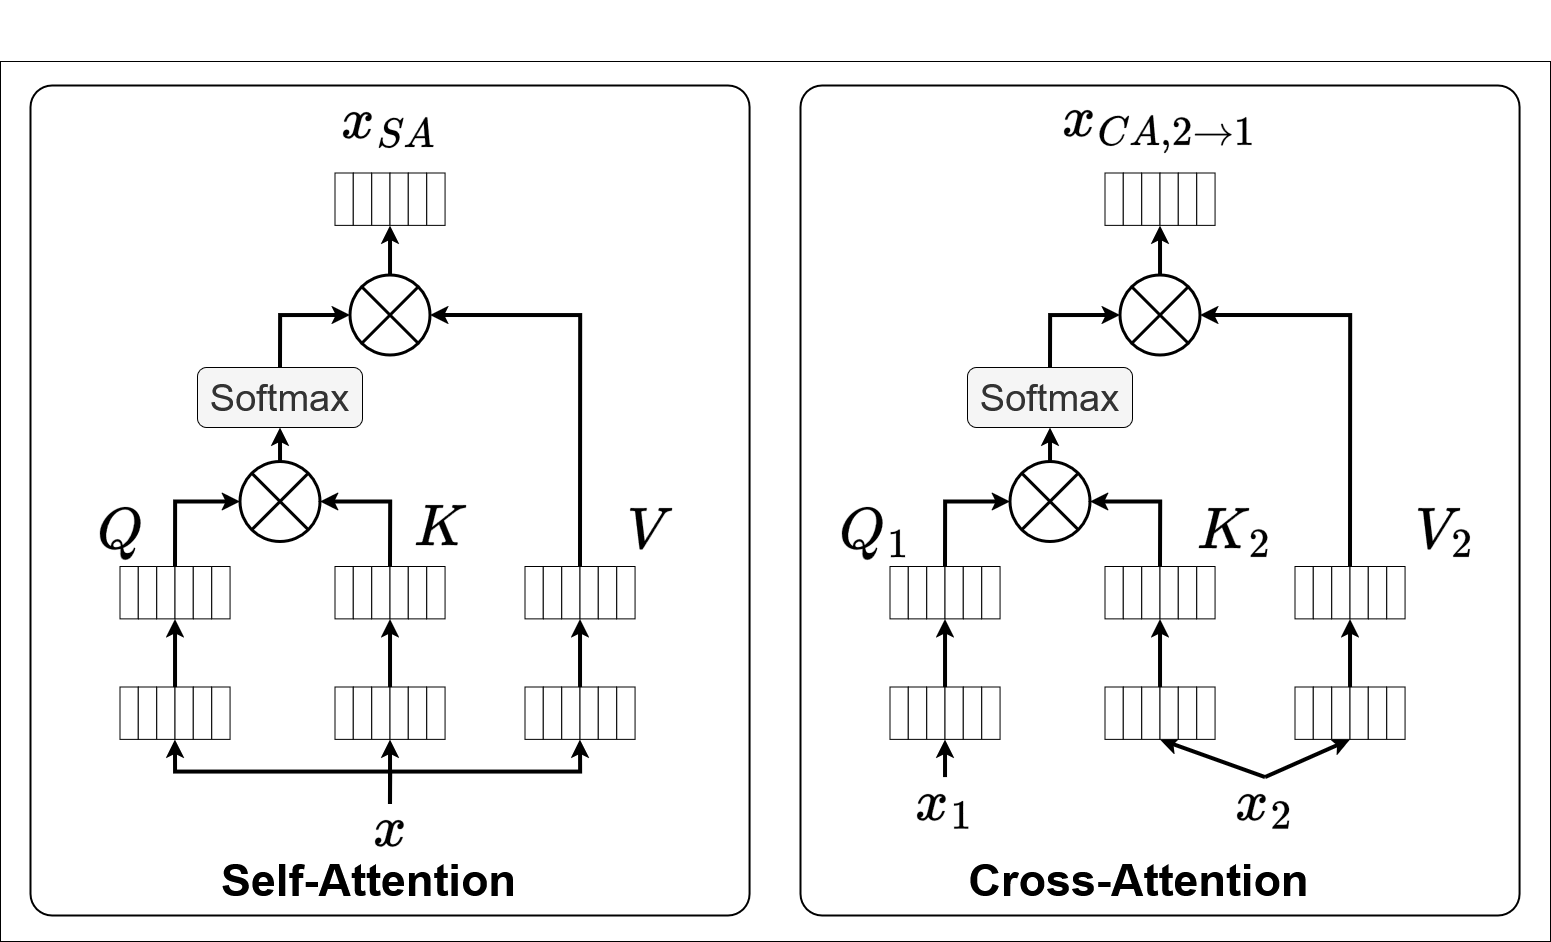
\includegraphics[width=0.9\linewidth]{figures/attention_diagram_simple}
  \caption{Attention allows models to extract and weight sections of an image during processing. Typically, two forms of attention are used, self-attention (left) and cross-attention (right).
  }
  \label{fig:bkgd-attn_example}
\end{figure}

%Attention \cite{} deserves its own introduction, both for its existing impact and for the role it plays in improved multi-view OOD detection. In general, there are two types of attention: self-attention and cross-attention. All attention mechanisms operate on a patch-style input format. Note that here we only consider image-based attention. That is, given an input image $x \in \mathbb{R}^{H \times W \times C}$, it is reshaped to have $T$ patches each of $d$ dimension, $x \in \mathbb{R}^{T \times d}$ where $d = P^2 \cdot C$ for patch resolution $P$. For an image input, this is analogous to sectioning the image $x$ into a grid of square image subsections of size $P$ before rearranging the sections into a sequence of $T$ length. Transformer models additionally prepend a class patch $x^0$ to the sequence and add position encoding to the patches \cite{dosovitskiy2020image}.
The Attention \cite{vaswani2017attention} mechanism has recently become a critical component in state-of-the-art neural network (NN)-based deep learning models \cite{dosovitskiy2020image}. There are two predominant types of attention: self-attention and cross-attention \cite{vaswani2017attention}. All attention mechanisms operate on a patch-style input format. Note that in this dissertation only image-based attention is considered. That is, given an input image $x \in \mathbb{R}^{\mathcal{I} \times \mathcal{J} \times \mathcal{K}}$ (where $\mathcal{I}, \mathcal{J}, \mathcal{K}$ refer to the image channel, width, and height dimensions respectively), traditionally the image is reshaped to have $T$ patches each of $d$ dimension, $x \in \mathbb{R}^{T \times d}$ where $d = P^2 \cdot \mathcal{I}$ for patch resolution $P$. For an image input, this is analogous to sectioning the image $x$ into a grid of square image subsections of size $P$ before rearranging the sections into a sequence of $T$ length. Transformer models additionally prepend a class patch $x^0$ to the sequence and add position encoding to the patches \cite{dosovitskiy2020image}. Examples of the types of attention, described below, can be found in \ref{fig:bkgd-attn_example}.

\textbf{Self-Attention:} An input $x$ is projected into a query $Q$, a key $K$, and a value $V$ using respective weight matrices $W_Q \in \mathbb{R}^{d \times d_k}$, $W_K \in \mathbb{R}^{d \times d_k}$, $W_V \in \mathbb{R}^{d \times d_v}$
\begin{equation}
\begin{aligned}
    Q & = x W_Q \\
    K & = x W_K \\
    V & = x W_V. \\
\end{aligned}
\end{equation}
$d_k$ and $d_v$ are projection dimensions selected by the user as hyperparameters. The query $Q$, key $K$, and value $V$ are used to calculate the attention as follows
\begin{equation}
\begin{aligned}
    \text{Attention}(Q,K) & = \text{softmax} (\frac{Q K^{\mathsf{T}}}{\sqrt{d_k}}) \\
    x_{SA}(\text{Attention},V) & = \text{Attention} \cdot V.
\end{aligned}
\end{equation}
%Attention effectively identifies which subsections of the image to attend to with respect to the optimization objective. The delineation of ``self-attention'' refers to the fact that the same input $x$ is used to compute each component ($Q$, $K$, $V$) for attention. Thus the attention mechanism references to and emphasizes components of itself when identifying important features. {\color{red}TODO; include figure showing what attention looks like} Self-attention can also be extended using multiple heads but this is out of scope of the dissertation \cite{vaswani2017attention}. The functionality is modular to any related method propositions.
Self-attention can also be extended to use multiple heads, but this is out of scope of the dissertation \cite{vaswani2017attention}.

\textbf{Cross-Attention:} Two inputs $x_1$ and $x_2$ are projected into a query $Q$, a key $K$, and a value $V$
\begin{equation}
\begin{aligned}
    Q & = x_1 W_Q \\
    K & = x_2 W_K \\
    V & = x_2 W_V, \\
\end{aligned}
\end{equation}
before attention is calculated as in self-attention
\begin{equation}
\begin{aligned}
    \text{Attention}(Q,K) & = \text{softmax} (\frac{Q K^{\mathsf{T}}}{\sqrt{d_k}}) \\
    x_{CA,2 \rightarrow 1}(\text{Attention},V) & = \text{Attention} \cdot V.
\end{aligned}
\end{equation}
